\documentclass[a4paper]{article}
\usepackage{color}
\usepackage{url}
\usepackage[T2A]{fontenc}
\usepackage[utf8]{inputenc} 
\usepackage{graphicx}
\usepackage{multirow}
\usepackage[english,serbian]{babel}
\usepackage[unicode]{hyperref}
\hypersetup{colorlinks,citecolor=red,filecolor=green,linkcolor=blue,urlcolor=blue}
\newtheorem{primer}{Primer}[section]

\begin{document}

\title{Virtuelna realnost\\ \small{Seminarski rad u okviru kursa\\Računarstvo i društvo\\ Matematički fakultet}}



\author{Jelena Čanković\\mi18096@alas.matf.bg.ac.rs}
\date{14. septembar 2022.}
\maketitle


\abstract {Virtuelna stvarnost i uređaji za reprodukciju virtuelne stvarnosti
\vspace{0.2cm}\\
\indent Definicija virtuelne stvarnosti dolazi od definicija obe reči „virtuelno“ i „stvarnost“. Definicija reči „virtuelno“ može značiti mnogo stvari, no vezana uz stvarnost, definisana je kao „bliska verzija stvarnosti“.\\
Ovim radom prisećamo se da svet spoznajemo isključivo kroz naša čula i mehanizme percepcije. Uređaji za reprodukciju virtualne stvarnosti, praćeni razvijenim softverom, proizvedeni su s namerom da zavaraju naša čula i pruže nam stvaran osećaj virtuelnog prostora. Nadalje, kroz rad se susrećemo s različitim iteracijama uređaja za reprodukciju virtuelne stvarnosti te opisujemo njihove karakteristike i kako pomoću njih korisnik komunicira tj. vrši interakciju s virtuelnom okolinom.} 
\vspace{0.2cm}\\
{\textbf{Ključne reči:}} virtuelna stvarnost, VR, interfejs, korisnik, vizuelno, oči, telo, sila, percepcija, pozicija, orijentacija, hardver, softver, sistemi, faza, performanse, robusnost, komunikacija, povratna informacija.


\tableofcontents
\vspace{1cm}
\section{Šta je Virtuelna realnost?}
\label{sec:šta je Virtuelna realnost?}
\indent{\textit{Reality is merely an illusion, albeit a very persistent one.}}
\begin{flushright}
{\textit{Albert Einstein}}}
\end{flushright}
\vspace{0.2cm}\\
\indent\quad Svedoci smo širenja Virtuelne realnosti, uzbudljive nove tehnologije koja obećava promenu načina na  koji interagujemo sa informacijama, prijateljima i svetom. To je medijum sa ogromnim potencijalom. Mogućnost da se korisnik transportuje na neko drugo mesto, potpuno uroni u iskustvo i oseća se kao da je stvarno prisutan, otvara nezamislive potencijale. Razvoj tehnologije doprineo je tome da VR uređaji budu pristupačni mnogobrojnim korisnicima.\cite{1}
\vspace{0.2cm}\\
\indent~Virtuelna realnost je kompjuterski generisana simulacija  $3$D prostora koja je korisniku dočarana veoma realno koristeći opremu sa senzorima za prostor. Cilj ove simulacije je stvaranje jakog osećaja prisutnosti u virtuelnom okruženju. Današnja VR oprema uključuje ''head-mounted display'' (HMD) - naočare za gledanje stereoskopskih $3$D scena (slika\ref{1}). Stereoskopija je tehnika kreiranja iluzije dubine na slici. Prikazuju se dve slike, za oba oka po jedna, koje su malo pomerene u stranu. Korisnik može gledati okolo pomeranjem glave i hodati korišćenjem ručnih kontrola i senzora za pokret. Potrošački hardver je nov i još se razvija. Međutim, nekoliko platformi je napravilo uređaje pristupačne korisnicima. Neki od njih su Oculus Rift, HTC Vive, Samsung Gear VR, Google Cardboard i Google Daydream.\\
\begin{figure}[!h]
\begin{center}
\includegraphics[scale=0.3]{1.1.jpg}
\label{1.1}
{\caption}
\end{center}
\end{figure}\\
\indent~Efekat virtuelne realnosti se postiže ,,varanjem''  ljudskog mozga, konkretno vizuelnog korteksa i delova mozga za percepciju pokreta. Mnoštvo tehnologija je uključeno u pravljenju ove iluzije kao što su: 
\begin{itemize}
\item~{\textbf{Stereoskopski ekrani.}} Poznati i kao $3$D ekrani ili HMD kombinuju dve slike, optičku distorziju i specijalna sočiva da naprave stereo sliku koju naš mozak interpretira kao trodimenzionalnu sliku.
\item~{\textbf{Hardver za praćenje pokreta.}} Žiroskopi, akselerometri i ostale komponente se koriste da prate pokrete tela i okrete glave kako bi aplikacija osvežila sliku u $3$D prostoru. 
\item~{\textbf{Uređaji za unos.}} Virtuelna realnost je donela potražnju za uređajima za unos koji su van domašaja tastature i miša. To su kontroleri i senzori za ruke i telo koji mogu da prepoznaju pokrete i gestove. 
\item~{\textbf{Desktop i mobilne platforme.}} Ovde spadaju kompjuterski hardver, operativni sistemi, softver za interfejs uređaja i softveri za pravljenje igara.
\end{itemize}

\section{Istorija i razvoj Virtuelne realnosti}
\label{sec:istorija i razvoj Virtuelne realnosti}
\indent~Virtuelna realnost je prisutna već decenijama i bila je korišćena u istraživačke, industrijske i vojne svrhe. U početku je bila jako glomazna i skupa.
\vspace{0.2cm}\\
\indent~U ranim devedesetim godinama pojavile su se prve stereoskopske slike i uređaj  ''View-Master'' (1993) koji je korišćen u turističke svrhe. Taj koncept se koristi za današnji Google Cardboard. Ivan Sutherland je 1968. godine napravio prvi HMD pod imenom ''The Ultimate Display''.\cite{2} Uređaj je bio veliki i isuviše težak da bi ga korisnik sam nosio. Zato je bio zakačen za plafon, a korisnik je morao da bude vezan za uređaj. Nakon toga bilo je nekoliko uređaja koji su bili ili preskupi ili neuspešni (EyePhone HRX\$49.000, SEGA VR Glasses, Nintendo Virtual Boy).\\
\indent Palmer Lakej i Džon Karmaksu pokrenuli kikstarter i objavili {\textbf{Oculus Rift Development Kit 1}} (DK1), komplet za razvoj virtuelne realnosti. Marta 2014. godine Fejsbuk je otkupio kompaniju za dva biliona dolara. Pažnja i novac koji su privučeni otvorili su novu kategoriju potrošačkih proizvoda. Nakon toga Google, Sony, Samsung i Steam su objavili svoje proizvode. Danas na tržištu imamo neke od poznatijih VR uređaja kao što su: Oculus Rift 2, HTC Vive, Playstation VR, Google Cardboard i Daydream i Samsung Gear VR. Iskustvo koje pružaju ovi uređaji kao i njihove  pojedinačne cene,  međusobno  se razlikuju. Uređaji su redom prikazani na slici \ref{2}.
\begin{figure}[!h]
\begin{center}
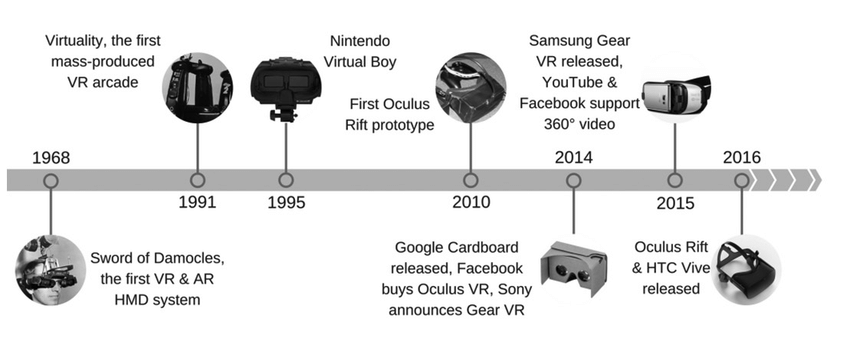
\includegraphics[scale=0.36]{2.png}
\label{2}
\end{center}
{\caption}
\end{figure}

\section{Tipovi naočara (Head-Mounted Display)}
\label{sec:tipovi naočara (Head-Mounted Display)}
\indent~Trenutno postoje dva tipa HMD-a za virtuelnu realnost. To su desktop VR i mobile VR. Svi HMD su povezani sa nekim uređajem, računarom, konzolom ili mobilnim telefonom.
\begin{itemize}
\item~{\textbf{Desktop VR.}} Ovde spadaju HMD uređaji koji su povezani kablovima na računare ili konzole koje imaju jače grafike. Igra se pokreće na mašini, a prikazuje se na HMD-u. Ovde spadaju Oculus Rift, HTC Vive i Playstation VR. 
\item~{\textbf{Mobile VR.}} Najjednostavniji primer mobile VR-a je Google Cardboard, jednostavno kućište (obično od kartona) sa dva sočiva i mestom za mobilni telefon. Telefon prikazuje dva stereografska prikaza i ima senzor za rotaciju glave, ali ne i za poziciju. Takođe postoji i dugme za klik kojim korisnik interaguje sa aplikacijom. Kvalitet i performanse su ograničene, jer aplikaciju pokreće procesor telefona. Pored Google Cardboard-a ovde spadaju i Samsung Gear VR i Google Daydream.\cite{4}
\end{itemize}

\section{Razlika između VR, AR i MR}
\label{sec:razlika između VR, AR i MR}
\indent~Pojmovi {\textbf{Virtual Reality}} i {\textbf{Augmented Reality}} se često mešaju. Kod VR-a korisnik je "prebačen" u virtuelni svet i kroz naočare ga vidi kao pravi svet. Augmented Reality (proširena realnost), skraćeno AR nadograđuje kompjuterski generisanu grafiku u realan svet. Primeri ovoga se mogu videti na mobilnim telefonima, tabletima i nekim ručnim konzolama kao što je Nintendo $3$DS. Jedna od najpoznatijih igara je Pokemon Go. Pored toga, AR se koristi i u muzejima. Najnoviji je pojam {\textbf{MR}} ili  {\textbf{Mixed (Merged) Reality}}. Microsoft je predstavio novi uređaj HoloLens, naočare koje povezuju VR i AR i prikazuje nadograđenu grafiku direktno u korisnikovom vidnom polju. 
\vspace{0.2cm}\\
\indent~Sve tri oblasti obećavaju dosta toga u budućnosti, ali različitog. Dok AR angažuje korisnika da interaguje sa trenutnom okolinom, virtuelna realnost u potpunosti uranja u novu okolinu i iskustvo. U AR možete na svom stolu stvoriti plan neke kuće, okretati ga i studirati, dok u VR možete ući u tu kuću i kretati se njom. HoloLens će omogućiti povezivanje ove dve stvari tako što će korisnik trenutno okruženje moći da pretvori u nešto sasvim novo po želji.\cite{3}
\begin{figure}[h!]
\begin{center}
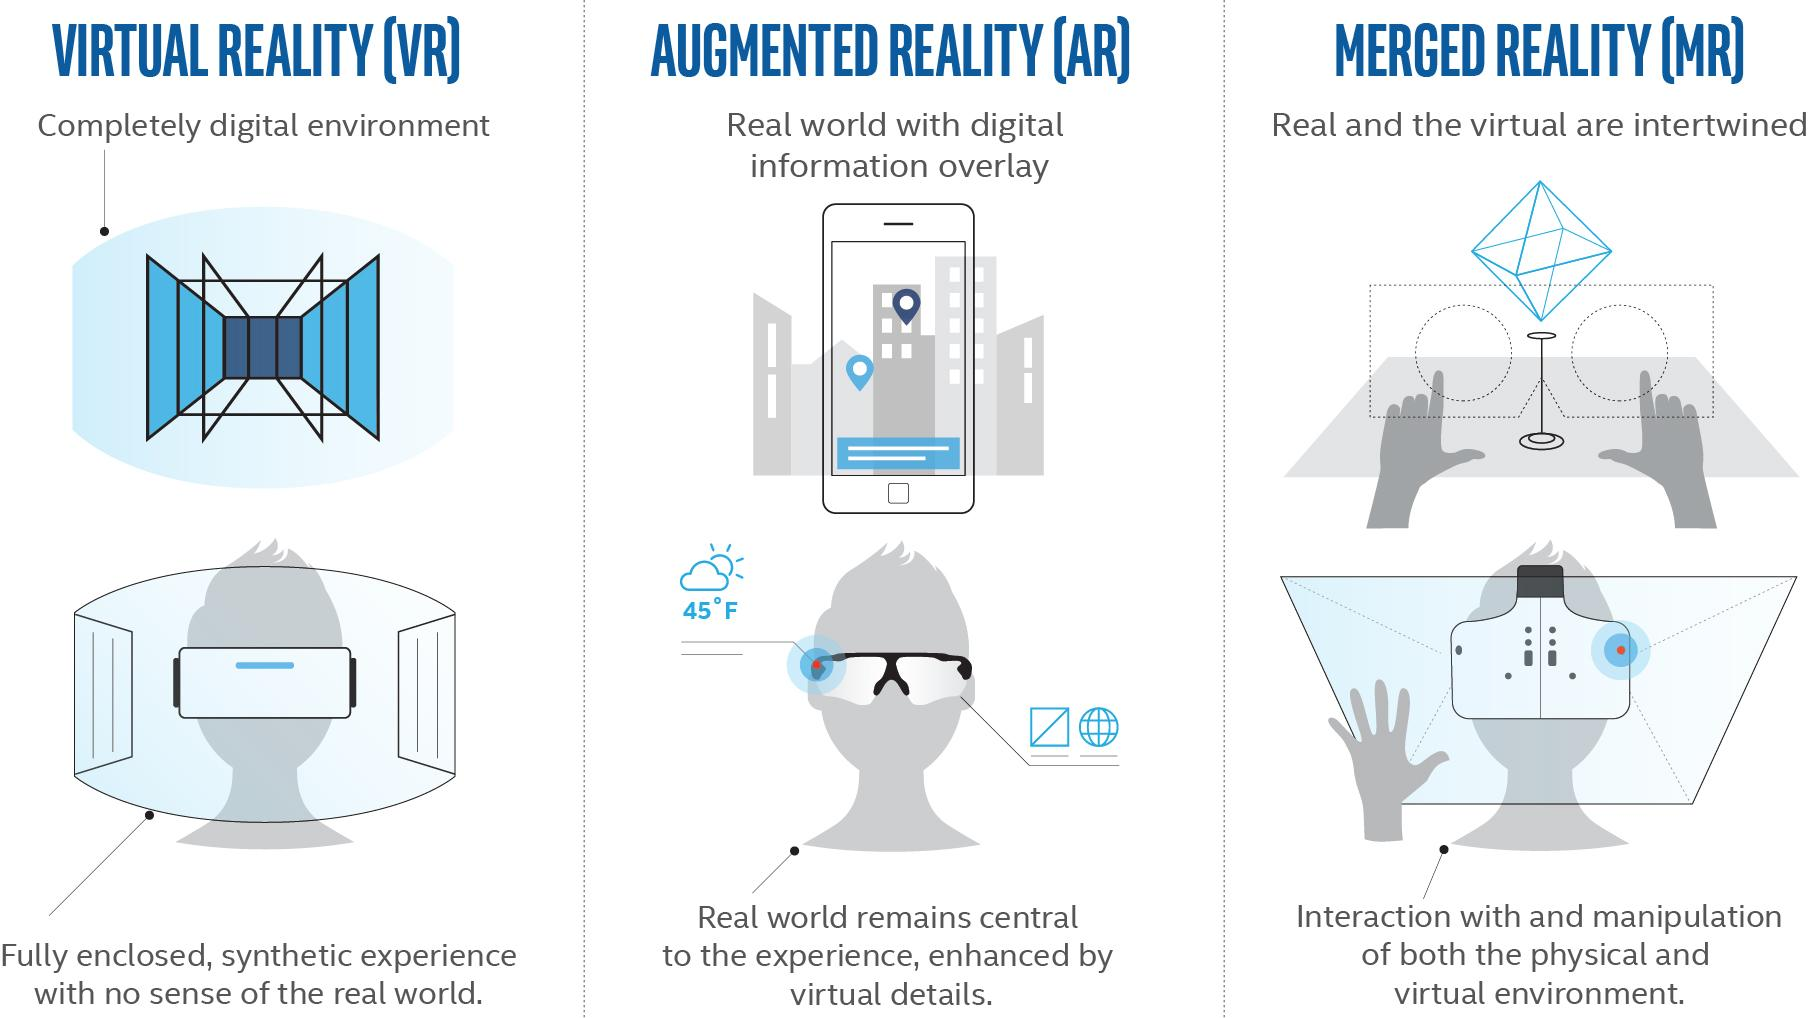
\includegraphics[scale=0.16]{3.jpg}
\label{3}
{\caption}
\end{center}
\end{figure}

\section{Povratna informacija}
\label{sec:povratna informacija}
\indent~Naš osećaj fizičke stvarnosti je konstruisan od simboličke, geometrijske  i dinamičke informacije, direktno prenete našim čulima. Virtuelni izlazni kanali stvarnosti stoga odgovaraju našim čulima: vid, dodir, miris, sluh, ukus i percepcija sile. Iz tog razloga, u srcu tehnologije virtuelne realnosti leži simulacija čula.\cite{1}

\subsection{Vizuelna percepcija}
\label{subsec:vizuelna percepcija}
\indent~Vid se generalno, s obzirom na njegovu osetljivost, smatra najdominantnijim čulom i postoje dokazi koji upućuju na to da je ljudska kognitivnost orijentisana oko vida. Visoko kvalitetna reprodukcija slike je iz tog razloga od najveće važnosti kada je reč o virtuelnom okruženju. Glavni aspekti koji utiču na ukupan kvalitet vizualnog utiska kod korisnika su sledeći:
\begin{itemize}
\item~Percepcija dubine
\item~Ugao vizuelne prostorne pokrivenosti
\begin{figure}[h!]
\begin{center}
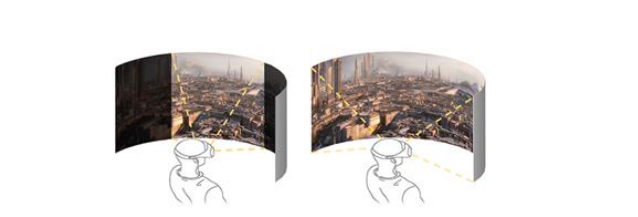
\includegraphics[scale=0.75]{4.png}
\label{4}
\caption{Prostorna pokrivenost}
\end{center}
\end{figure}
\item~Kritična frekvencija stapanja slike
\end{itemize}\\


\subsection{Percepcija zvuka}
\label{subsec:percepcija zvuka}
\indent~Generalno analizirajući čula, možemo reći da je vid naše primarno čulo. Sluh većinom koristimo za verbalnu komunikaciju, kako bismo dobili informaciju iz očima nedostupnog prostora, odnosno kada oči ne pružaju dovoljno informacija. Zvukom se koristimo da bi u prostoru pozicionirali izvore te se može povezati s generatorom govora za verbalnu komunikaciju s računarom. Kod ljudi, slušni organ je najefikasniji između $1000$  i $4000~\mathrm{Hz}$, s padom efikasnosti pređe li frekvencija gornju ili donju granicu. Prostorna orijentacija se svodi na razliku udaljenosti između ušiju i izvora zvuka. Ovim internim navođenjem se koristimo pri određivanju azimutalne usmerenosti (levo ili desno), koje je vrlo precizno. Spoznajom o tim svojstvima, moguće je proizvesti $3$D zvučne sisteme koji poseduju neka zanimljiva svojstva, kao što su: simulacija Dopplerovog pomaka dok objekt putuje pored slušaoca, kontrola kontinuiranih zvukova, mogućnost ultrazvučnog mapiranja prostorije i druga.

\subsection{Percepcija sile, dodir i pozicija}
\label{subsec:percepcija sile, dodir i pozicija}
\indent~Čulo vida i mirisa koristimo samo za opažanje, no čulo dodira je sposobno osetiti šta se događa u okolini ljudskog bića, ali i delovati na okolinu. Iz tog  razloga dodir je neizostavan  deo mnogih ljudskih aktivnosti za koje VR što realnije mora pružiti ulazne kanale i manifestovati izlazne kanale. Primarne ulazno/izlazne varijable čula dodira su deformacije i sile. Ulazne informacije se dele na dodirne i vizuelne, a razlikuju se u sledećem. Ako ruka obuhvati određeni objekt, prvi osećaj je dodir receptora kože koji nam prenosi informaciju o obliku i teksturi objekta. Ako ruka prinese više sile, pristižu nam vizuelne informacije o poziciji i pokretu šake i ruke te sile koje deluju na njih, kao i informacije o površinskoj popustljivosti, a ne retko i težini. Da bi se objektom manipulisalo, da bi se pomerilo, rotiralo ili pak uštipnulo, sistem mora izdati naredbu motorima koji vrše silu na objekt. Snažni stisak se postiže vršenjem sile prstima i dlanom, a precizno hvatanje se vrši koristeći samo vrhove prstiju. Dva glavna aspekta kod simulacije silom koji utiču na zahteve VR-a su maksimalna veličina sile i frekvencija povratne informacije.

\subsection{Percepcija mirisa}
\label{subsec:percepcija mirisa}
\indent~ Glavni problem kod simulacije ljudskog čula mirisa leži u činjenici da su mnoga pitanja o tome kako on zapravo radi ostala neodgovorena. Jasno je da su molekuli koje prenose mirise u nosu uhvaćeni od strane receptorskih neurona, ali je nejasno kako mozak generiše uzorke za prepoznavanje, pri čemu izoluje jedne određene mirise od drugih i rekonstruiše ono što nedostaje. Dokazano je  da čovek može njuhom identifikovati oko trećinu mirisa, u neprisustvu drugih čula, kao na primer vida. S druge strane, ljudska sposobnost detekcije mirisa je vrlo osetljiva. Takođe, lakše je detektovati porast koncentracije nekog mirisa, nego pad te koncentracije. VR uređaj koji bi pružao korisniku čulo mirisa, mora takođe pružiti i mogućnost filtriranja vazduha.\cite{1}
\begin{figure}[h!]
\begin{center}
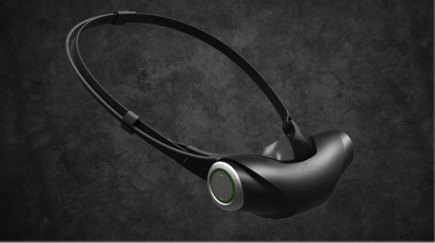
\includegraphics[scale=0.63]{5.png}
\label{5}
\end{center}
\caption{Uređaj za simulaciju čula mirisa sa izmenjivim mirisnim kapsulama}
\end{figure}

\section{Hardverska rešenja za doživljaj virtuelne stvarnosti}
\label{sec:hardverska rešenja za doživljaj virtualne stvarnosti}
\indent~Trenutno se na tržištu  mogu naći različiti uređaji za doživljaj virtuelne stvarnosti. Neki od njih su VR naočare, $3$D zvučni sistemi, uređaji za detekciju pokreta svakog dela tela, sistemi za mapiranje prostorija (laserski i ultrazvučni), govorni sintetizatori, uređaji za prepoznavanje govora, pa čak i uređaji za ispuštanje mirisa, sve kako bi se u potpunosti prepustili nesvakidašnjosti virtuelne stvarnosti.

\subsection{Praćenje pozicije/orijentacije}
\label{subsec:praćenje pozicije / orijentacije}
\indent~U VR sistemima, praćenje položaja glave je najvažnija ulazna informacija kada je reč o uranjanju u virtuelnu stvarnost. Uređaji koji se koriste za praćenje položaja glave se takođe mogu implementirati za praćenje položaja drugih delova tela (rukavice, odelo). Mnogo je tehnologija koje se koriste za prostorno praćenje delova tela. Mehanički sistemi mere promene pozicije i fizički povezuju  udaljeni objekat  na referentnu tačku spojnim vezama. Vrlo su precizni, imaju malo kašnjenje i zgodni su za praćenje objekata s malim volumenom, no podložni su mehaničkom trošenju materijala. Magnetske sisteme čine parovi odašiljača magnetnog polja i prijemnika, sposobnih da utvrde kojom snagom i pod kojim uglom na njih deluje polje. Relativno su jeftini i precizni, no podložni su distorzijama polja i elektromagnetskoj interferenciji.  Optički sistemi mogu koristiti raznovrsne optičke detektore za detektovanje ambijentalne rasvete ili svetla emitovanog od strane uređaja za praćenje pozicije (uobičajeno je da se koristi infracrveno svetlo kako bi se izbegla interferencija s drugim izvorima). Rade na relativno velikim područjima i nisu podložni smetnjama, ali su teški i skupi.\cite{5}
\begin{figure}[h!]
\begin{center}
\includegraphics[scale=0.63]{6.png}
\label{6}
\end{center}
{\caption}
\end{figure}

\subsection{Praćenje očiju}
\label{subsec:praćenje očiju}
\indent~Uređaji za praćenje očiju rade nešto drugačije. Ne mere poziciju ni orijentaciju glave, već detektuju smer u kojem gledaju oči korisnika u zadanom trenutku. Ova se informacija koristi kako bi se u realnom vremenu zaslon prilagodio korisniku. Uređaji za praćenje pogleda očiju realizovani  su na više načina: optički, elektrookularno i elektromagnetski. Komercijalno najrašireniji su optički uređaji koji koriste infracrveno LED (engl. Light Emitting Diode) svetlo kako bi osvetlili oko, pri čemu je generisana refleksija na rožnjači pomoću koje se ustanovi smer gledanja korisnika.\cite{6}


\subsection{Kretanje celog tela}
\label{subsec:vizuelna percepcija}
\indent~Pod kretanjem celog tela podrazumevamo dva načina kretanja: pasivno i aktivno samokretanje. Pasivno kretanje se izvodi simulacijom vozila određene tehnologije. Uobičajena praksa je izgradnja kabine koja predstavlja fizičko vozila i njegove kontrole, te se postavlja na pokretnu platformu sa zaslonima koji reprodukuju virtuelnu okolinu. Okolina se menja u odnosu na uticaj korisnika. Ovakve se instalacije specijalno koriste za simulatore leta i predstavljaju prvu praktičnu VR primenu za vojne pilote prilikom obuke, a u poslednje se vreme ova tehnologija sve više primjenjuje i u svrhu zabave.


\subsection{VR naočare}
\label{subsec:vr naočare}
\indent~\textbf{Oculus Rift}} je vizualni interfejs za prikaz virtuelne stvarnosti, proizveden od strane „Oculus VR-a“, a u prodaji je od $2016$. Rift je pre finalne verzije prošao kroz mnoge faze razvoja, od kojih je pet bilo predstavljeno javnosti. Sadrži OLED (engl. organic light-emitting diode) zaslon, podržava rezoluciju od $1080\times1200$ po oku, te pri brzini osvežavanja od $90~\mathrm{Hz}$  pruža $110^{\circ}$ prostorne pokrivenosti. Ima integrisane slušalice s podržanim $3$D efektom te pruža praćenje pozicije i rotacije. Sistem za praćenje pozicije, nazvan  ''Constellation''  izveden je USB (engl. Universal Serial Bus) stacionarnim infracrvenim senzorom koji ubire svetlo emitovano od strane IR LED dioda, integrisanih u sučelju. Senzor je uobičajeno postavljen na korisnikovoj radnoj površini, pa stvara $3$D prostor u kojem omogućuje korisniku upotrebu Rifta sedeći, stojeći ili pak hodajući kroz prostoriju.\cite{7}\\
\begin{figure}[h!]
\begin{center}
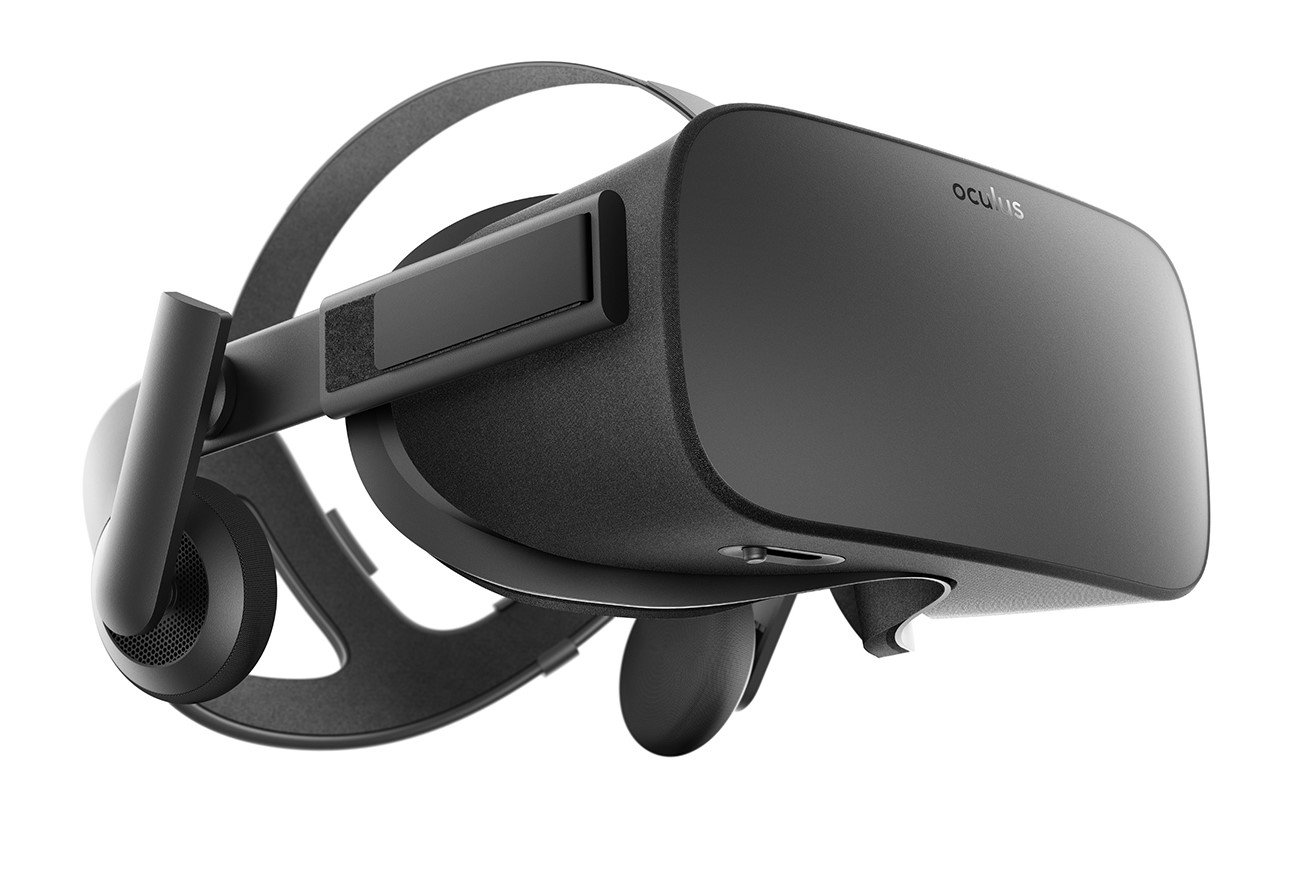
\includegraphics[scale=0.2]{7.jpg}
\label{7}
\caption{Oculus}
\end{center}
\end{figure}\\
\indent~{\textbf{PlayStation VR}} je sučelje za virtualnu stvarnost koje proizvodi Sony kompanija, pa je namenjeno  konzoli  za igranje ''PlayStation 4''.\cite{8}
\vspace{0.2cm}\\
\indent~{\textbf{HTC Vive}} je, po mnogima, trenutno najbolje VR vizualno sučelje na tržištu. Malo teže je uporediti ga s Oculus Riftom i PSVR-om, međutim to postaje u potpunosti neprimetno jednom kada se uroni u Vive-ov virtuelni svet. Rezolucija koju Vive podržava je $2160\times1200$ na OLED zaslonu pri brzini osvežavanja od  $90~\mathrm{Hz}$, a ugao prostorne pokrivenosti iznosi  $110^{\circ}$.
\vspace{0.2cm}\\
\indent~{\textbf{Mcrosoft HoloLens}} interfejs je uređaj koji izgledom podseća na sunčane naočare, ali je zapravo  prozor u svet proširene stvarnosti (engl. augmented reality). Ovo je prvi, individualni holografski računar. Sastavljene su  od specijalizovanih komponenti koje omogućavaju veliku obradu podataka u kratkom vremenu, pa  pružaju nesmetano kretanje i interakciju korisnika s hologramima.\cite{9}


\section{Zaključak}
\label{sec:zaključak}
\indent~Od kako je predstavljena široj javnosti, virtuelna stvarnost privlači pažnju velikog broja kako istraživača tako i korisnika. 
S razvojem tehnologije virtuelna stvarnost se razvija i pruža sve kvalitetnije usluge. U početku se koristila isključivo na području igrica, dok sad svoju primenu nalazi u različitim sferama života. Naučnici kao i korisnici očekuju sve veću primenu virtuelne stvarnosti u svakodnevnici, kao i njen sve veći napredak.
\newpage
\addcontentsline{toc}{section}{Literatura}
\begin{thebibliography}{99}
\bibitem{1}Virtual Reality: Scientific and
Technological Challenges (1995) -\\ Nathaniel I. Durlach and Anne S. Mavor, Editors
\bibitem{2}Sutherland, I. E., ''The ultimate display'', Vol. 2, pp. 506–508
\bibitem{3}Carr, K., England, R., ''Simulated and Virtual Realities''
\bibitem{4}Fisher, S. S., Mcgreevy, M., Humphries, J., Robinett, W., ''Virtual environment display system''
\bibitem{5}Gobbetti, E., Balaguer, J., ''An integrated environment to visually construct 3D animations''
\bibitem{6}Davson, H., ''Physiology of the Eye''
\bibitem{7}{\href{https://en.wikipedia.org/wiki/Oculus\_Rift}{https://en.wikipedia.org/wiki/Oculus\_Rift}
\bibitem{8}{\href{http://www.cnet.com/products/sony-playstation-vr/}{http://www.cnet.com/products/sony-playstation-vr/}
\bibitem{9}{\href{http://www.techradar.com/reviews/wearables/microsoft-hololens-1281834/review}{http://www.techradar.com/reviews/wearables/microsoft-hololens-1281834/review}

\end{thebibliography}
\end{document}